\subsubsection{Data Description and Preprocessing}
Atac-Seq is an emerging evoluted technique which enables to investigate the open chromatin regions at whole genome level.
It has been demonstrated the adequacy of this technology in the regulation of mouse brain activity under different conditions.

To illustrate the performances of \gls{descan} we chose a dataset \cite{Su2017} that describes in vivo adult mouse dentate granule neurons before and after synchronous neuronal activation using Atac-Seq and RNA-Seq technologies (see sections \ref{sec:atacseq} and \ref{sec:rnaseq} for a description of these sequencing techniques).

This dataset is organized in 62 samples of Atac-Seq and RNA-Seq, extracted at four different time points (0, 1h, 4h, 24h), with four replicates at each time point.
We chose to compare the differences btween the first two stages, time 0 (E0) and 1 hour after neuronal induction (E1), in order to show a potential Atac-Sec workflow for Differential Enrichment, and how to integrate this data type with RNA-Seq. A general illustration of this dataset is represented in figure \ref{fig:atacdataset}.

\begin{figure}[H]
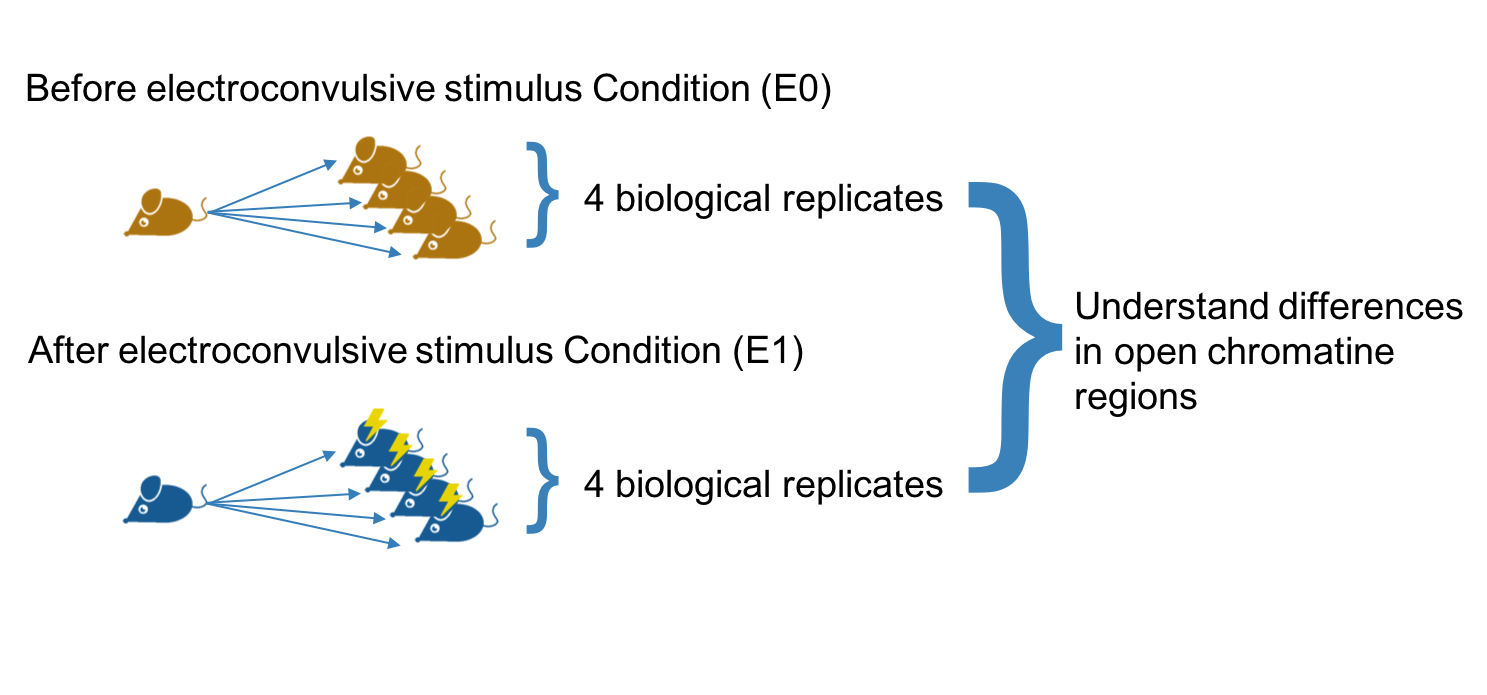
\includegraphics[width=\textwidth,height=\textheight,keepaspectratio]{img/descan2/dataset.png}
\caption[DEScan2 dataset illustration]{An illustration of our extraction of the GSE82015\cite{Su2017} dataset.}
\label{fig:atacdataset}
\centering
\end{figure}

We downloaded the data from \gls{geo} database \cite{Edgar2002, Barrett2013} with accession number GSE82015\footnote{\url{https://www.ncbi.nlm.nih.gov/geo/query/acc.cgi?acc=GSE82015}} and mapped raw data using \textit{STAR} \cite{Dobin2013} with default parameter on \gls{mm10}.

\subsubsection{Peaks Detection}

In order to detect open chromatin regions we run our peak caller, cutting the genome in bins of 50bp and using running windows of minimum 50bp and maximum 1000bp. In such a way we are able to detect not just broad peaks, but also smaller peaks.

To be confident with our results we run \gls{descan} and \textit{MACS2} on the same samples, and (as shown in figure \ref{fig:des2m2peaks}) looking to the numbers \gls{descan} always outperforms \textit{MACS2} peaks.

\begin{figure}[H]
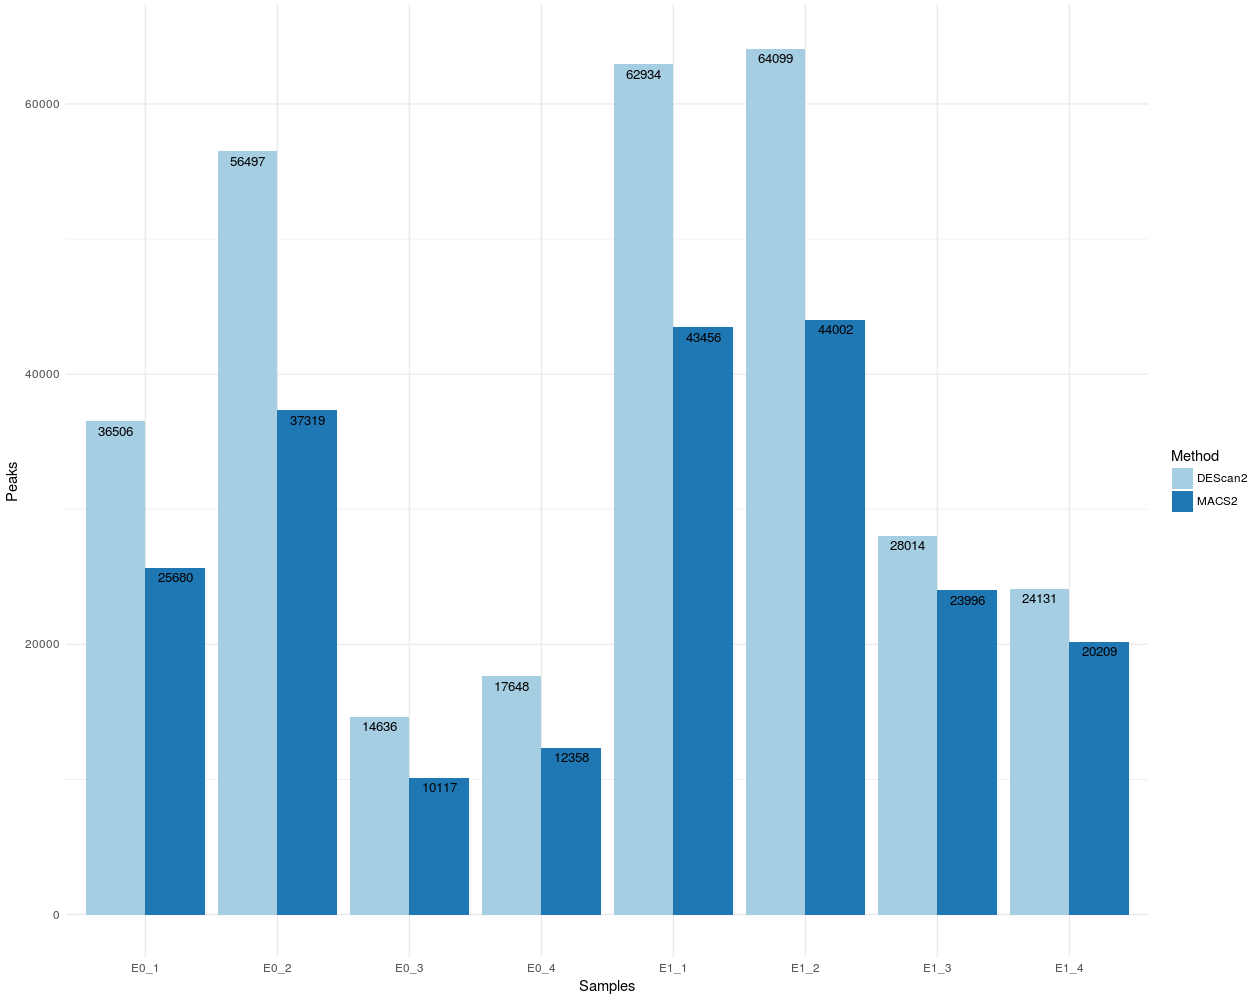
\includegraphics[width=\textwidth,height=\textheight,keepaspectratio]{img/descan2/d2m2_peaks_number.png}
\caption[The \gls{descan} and \textit{MACS2} peaks detection]{A comparison of \gls{descan} and \textit{MACS2} detected peaks for each sample in the dataset.}
\label{fig:des2m2peaks}
\centering
\end{figure}

To be more robust, we compared \gls{descan} detected peaks with the same validated regions (\textit{Arc}\footnote{https://www.genecards.org/cgi-bin/carddisp.pl?gene=ARC} and \textit{Gabrr1}\footnote{https://www.genecards.org/cgi-bin/carddisp.pl?gene=GABRR1}) of the original work \cite{Su2017}.
The lower part of figure \ref{fig:peaksdescan} shows the detected and validated regions (in blue and red) resulting differentially enriched between the E0 (in pink) and E1 (in green) conditions, while the upper part shows \gls{descan} filtered and aligned peaks (in blue) between the samples, highlighting a capability to catch not only the same regions of the published ones, but also (gold circles) to be more careful in the smaller peaks detection.

\begin{figure}[H]
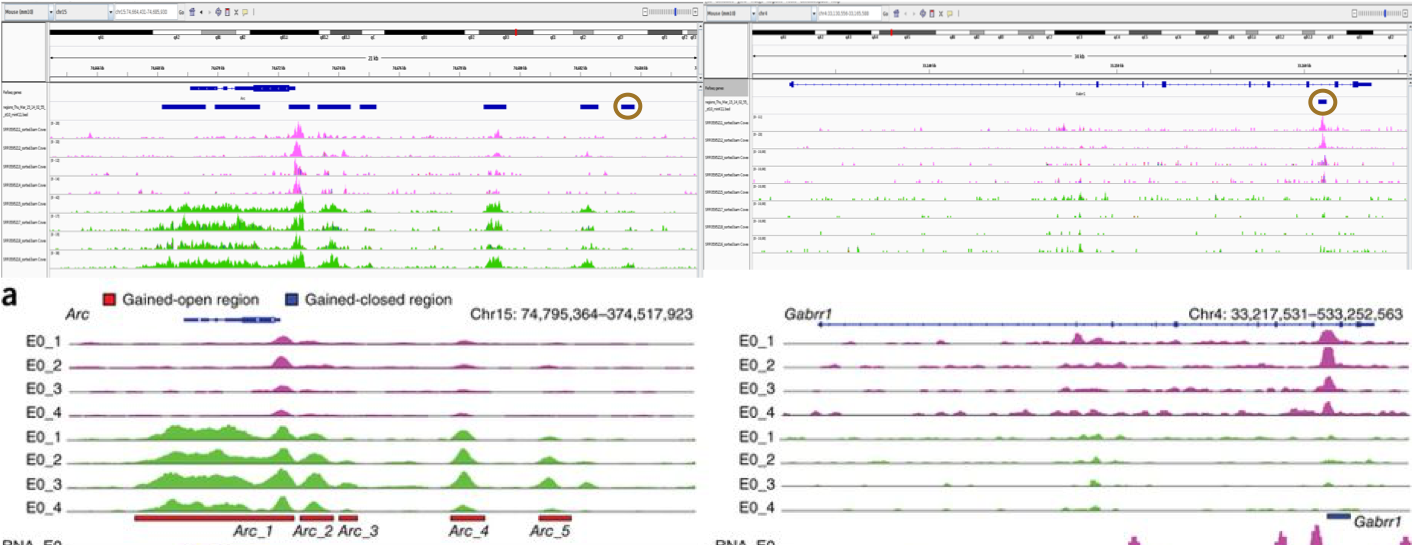
\includegraphics[width=\textwidth,height=\textheight,keepaspectratio]{img/descan2/peaks.png}
\caption[\gls{descan} peaks detection]{A comparison of \gls{descan} detected peaks with validated peaks in article \cite{Su2017}.}
\label{fig:peaksdescan}
\centering
\end{figure}

\subsubsection{Removing Unwanted Peaks}

While it is very important to detect good peaks with a peak caller, it seems to be more relevant to detect reliable regions. Indeed, during the filtering/aligning step, the number of peaks depends not only by the peak score, but also by the number of replicates designed in the experiment.
The figure \ref{fig:filteringdescanmacs2} puts in relation these two relevant information for both MACS2 and \gls{descan}. 
On the x-axis is represented the number of replicates, while on the y-axis is traced the number of peaks, and each curve represents a different threshold on the peaks score, showing that higher are the thresholds on the scores and the number of replicates, lower is the number of the detected peaks.
Highlighting a proportional inversion between the number of the peaks and the combination of the number of samples and the detected regions score.
%\begin{figure}[H]
%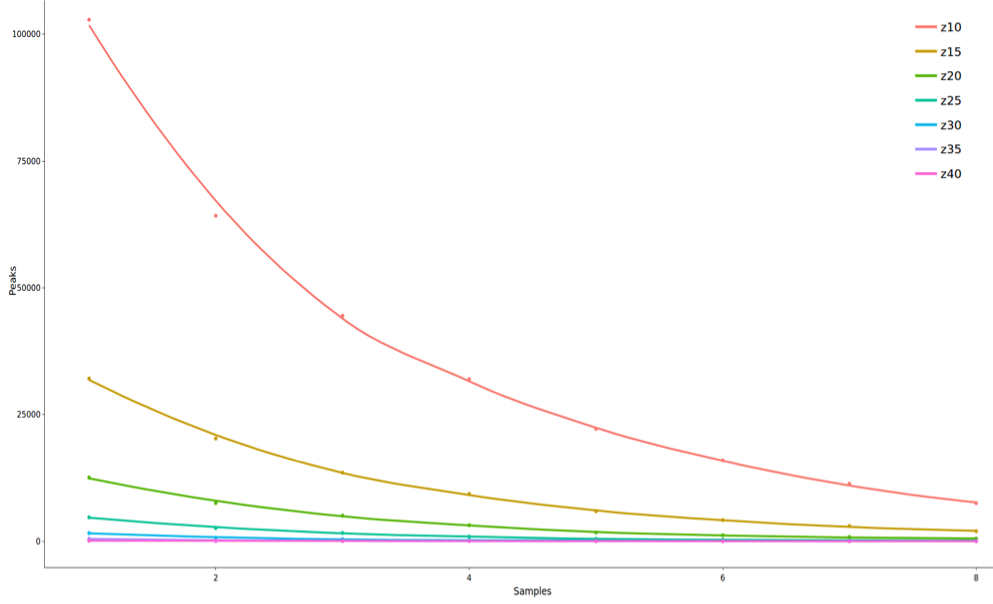
\includegraphics[width=\textwidth, height=\textheight, keepaspectratio]{img/descan2/filtering.png}
%\caption[\gls{descan} filtering step]{Filtering the detected regions with different thresholds on peak scores.}
%\label{fig:filteringdescan}
%\centering
%\end{figure}

\begin{figure}[H]
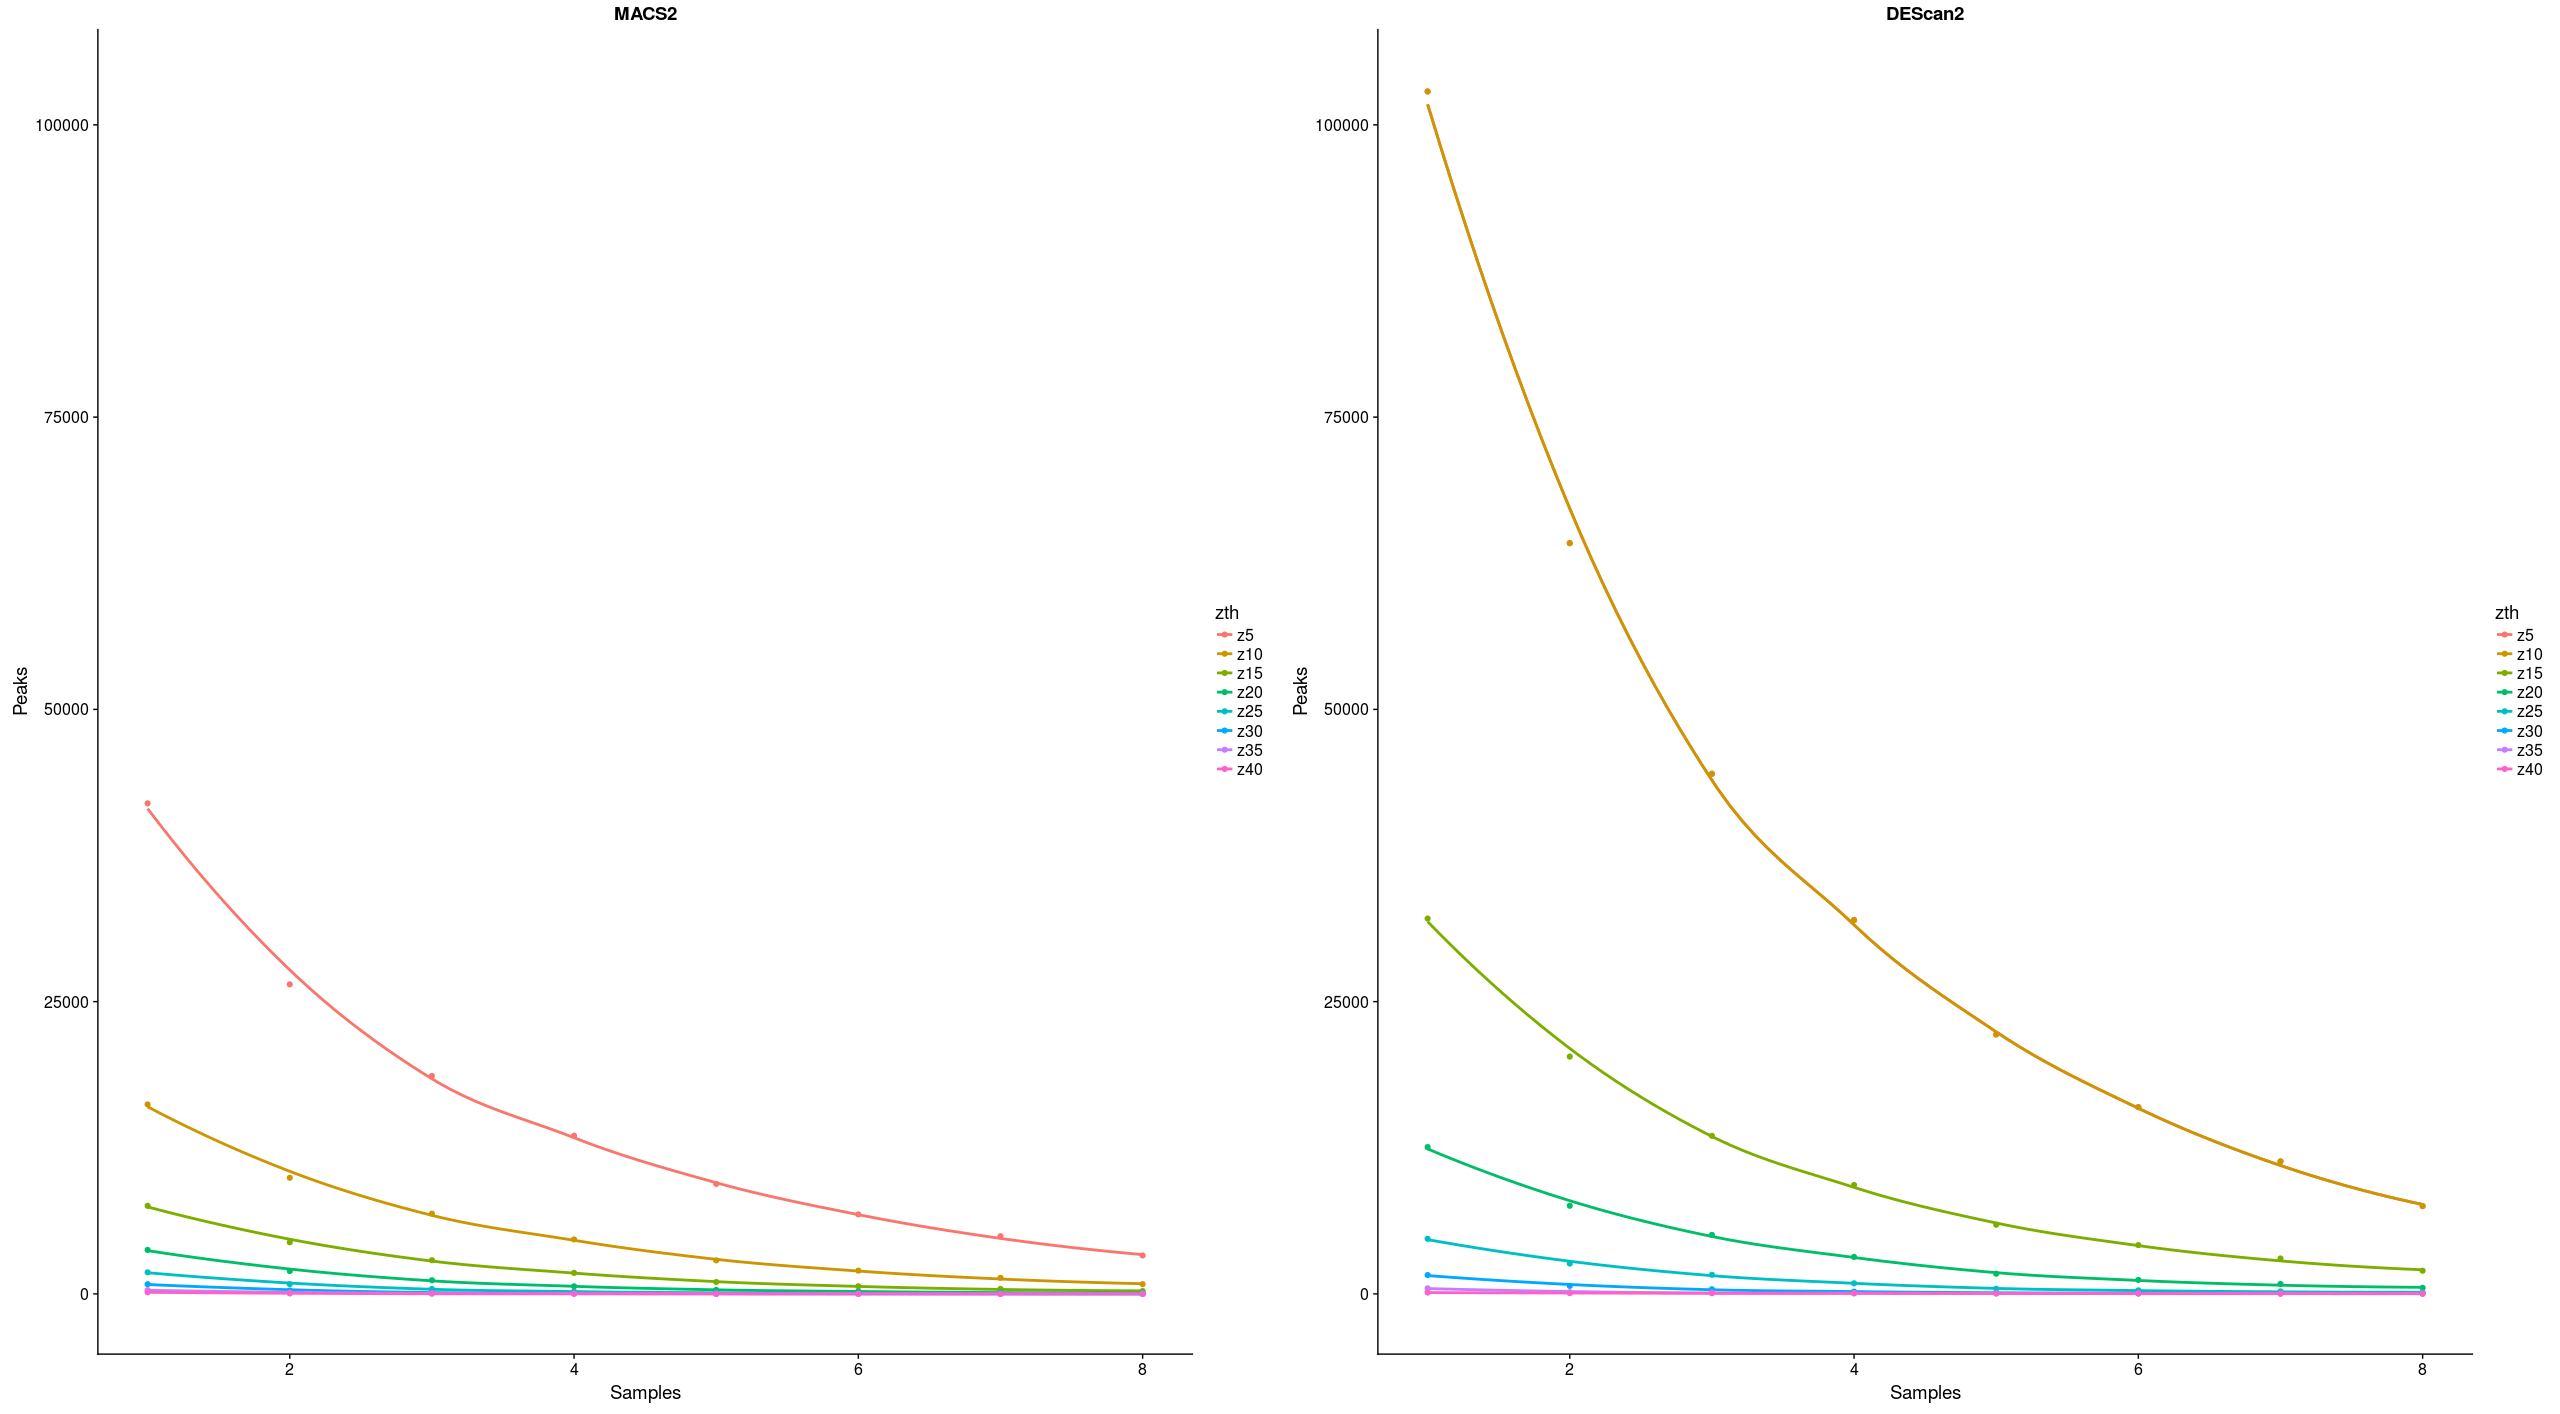
\includegraphics[width=\textwidth, height=\textheight, keepaspectratio]{img/descan2/filtering_m2_d2.png}
\caption[\gls{descan} and \textit{MACS2} filtering comparison]{Filtering the detected regions with different thresholds on peak scores between \textit{MACS2} and \gls{descan}.}
\label{fig:filteringdescanmacs2}
\centering
\end{figure}


Moreover, comparing left and right panels, we notice the high difference in pooling the samples-peaks together with the \gls{descan} filtering/aligning step when using the \textit{MACS2} and the \gls{descan} peaks.
Using the \textit{MACS2} peaks the pooling highly reduce the number of detected peaks, even using a low threshold as 5 on the score, showing that there are many peaks with a score lower than 5.
While in the \gls{descan} case the curves representing the threshold equal to 5 and the threshold equal to 10 totally overlap, highlighting that the \gls{descan} peak caller produces scores higher than 10.

\subsubsection{Quantifying Peaks}

Afterwards, the filtered-in regions can be processed by \gls{descan} in order to obtain a count matrix with samples on the columns and peaks on the rows.
This type of data structure is very versatile, because it enables to perform several operations, like the \glspl{der} and the integration with other kind of omics, as RNA-Seq.

\begin{figure}[H]
\centering
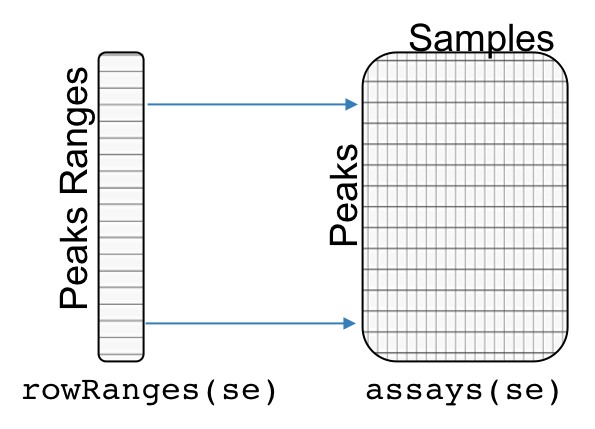
\includegraphics[scale=.7]{img/descan2/counts.png}
\caption[\gls{descan} counts illustration]{An illustration of the \textit{SummarizedExperiment} data structure produced by \gls{descan}.}
\label{fig:countsdescan}
\centering
\end{figure}

In order to preserve the information associated to the peaks, \gls{descan} produces as output a \textit{SummarizedExperiment} (figure \ref{fig:countsdescan}) data structure, which enables to retrieve the count matrix with \lstinline!assays! method, and to access the peaks information in \textit{GenomicRanges} format with the \lstinline!rowRanges! method.


\subsubsection{Peaks Normalization}

Before to proceed to detect \glspl{der}, it is a good standard to normalize the data, also because without any kind of normalization we are not able to detect any \gls{der}.
The nature of the data, in count format, makes it possible to apply several well known RNA-Seq normalizations techniques, such as \textit{TMM}, \textit{upper-quartile}, \textit{full-quantile}, \textit{RUV-Seq}, etc \cite{Risso2014h, Robinson2010, Dillies2013}.
In this case, we fixed the peaks's score threshold to 10, in order to have as much signal as possible.

While the \textit{TMM} and \textit{upper-quartile} normalizations modify the data in a way that makes it impossible to detect \glspl{der}, other kind of normalizations and combinantions of them give good results.

The figure \ref{fig:normalizationsnullfull} sintetizes this concept very well, highlighting a relation between the number of \glspl{der} (y-axis) and the minumum number of samples (x-axis) used for filtering the data during the \gls{descan} filtering step.

To better compare the normalization effect, we created a \textit{null dataset} of 8 samples, simply doubling the E0 samples and differentially express the signal between E0 (4 samples) and E0-fake (4 samples).

The right panel of the plot, representing the "full dataset", shows that \textit{upper-quantile}, even if combined with \textit{RUV-Seq} normalization, is not able to linearly detect a good amount of \glspl{der}, while \textit{full-quantile}, when combined with \textit{RUV-Seq} seems to affect the data in a way that overdetect the number of \glspl{der}. 
When looking at the \textit{full-quantile} and \textit{RUV-Seq} by themself seem to perform better than the other normalizations. The first one has a downhill almost linear, while the second one has a very fast downhill with a regrowth when the number of samples is higher.

\begin{figure}[H]
\centering
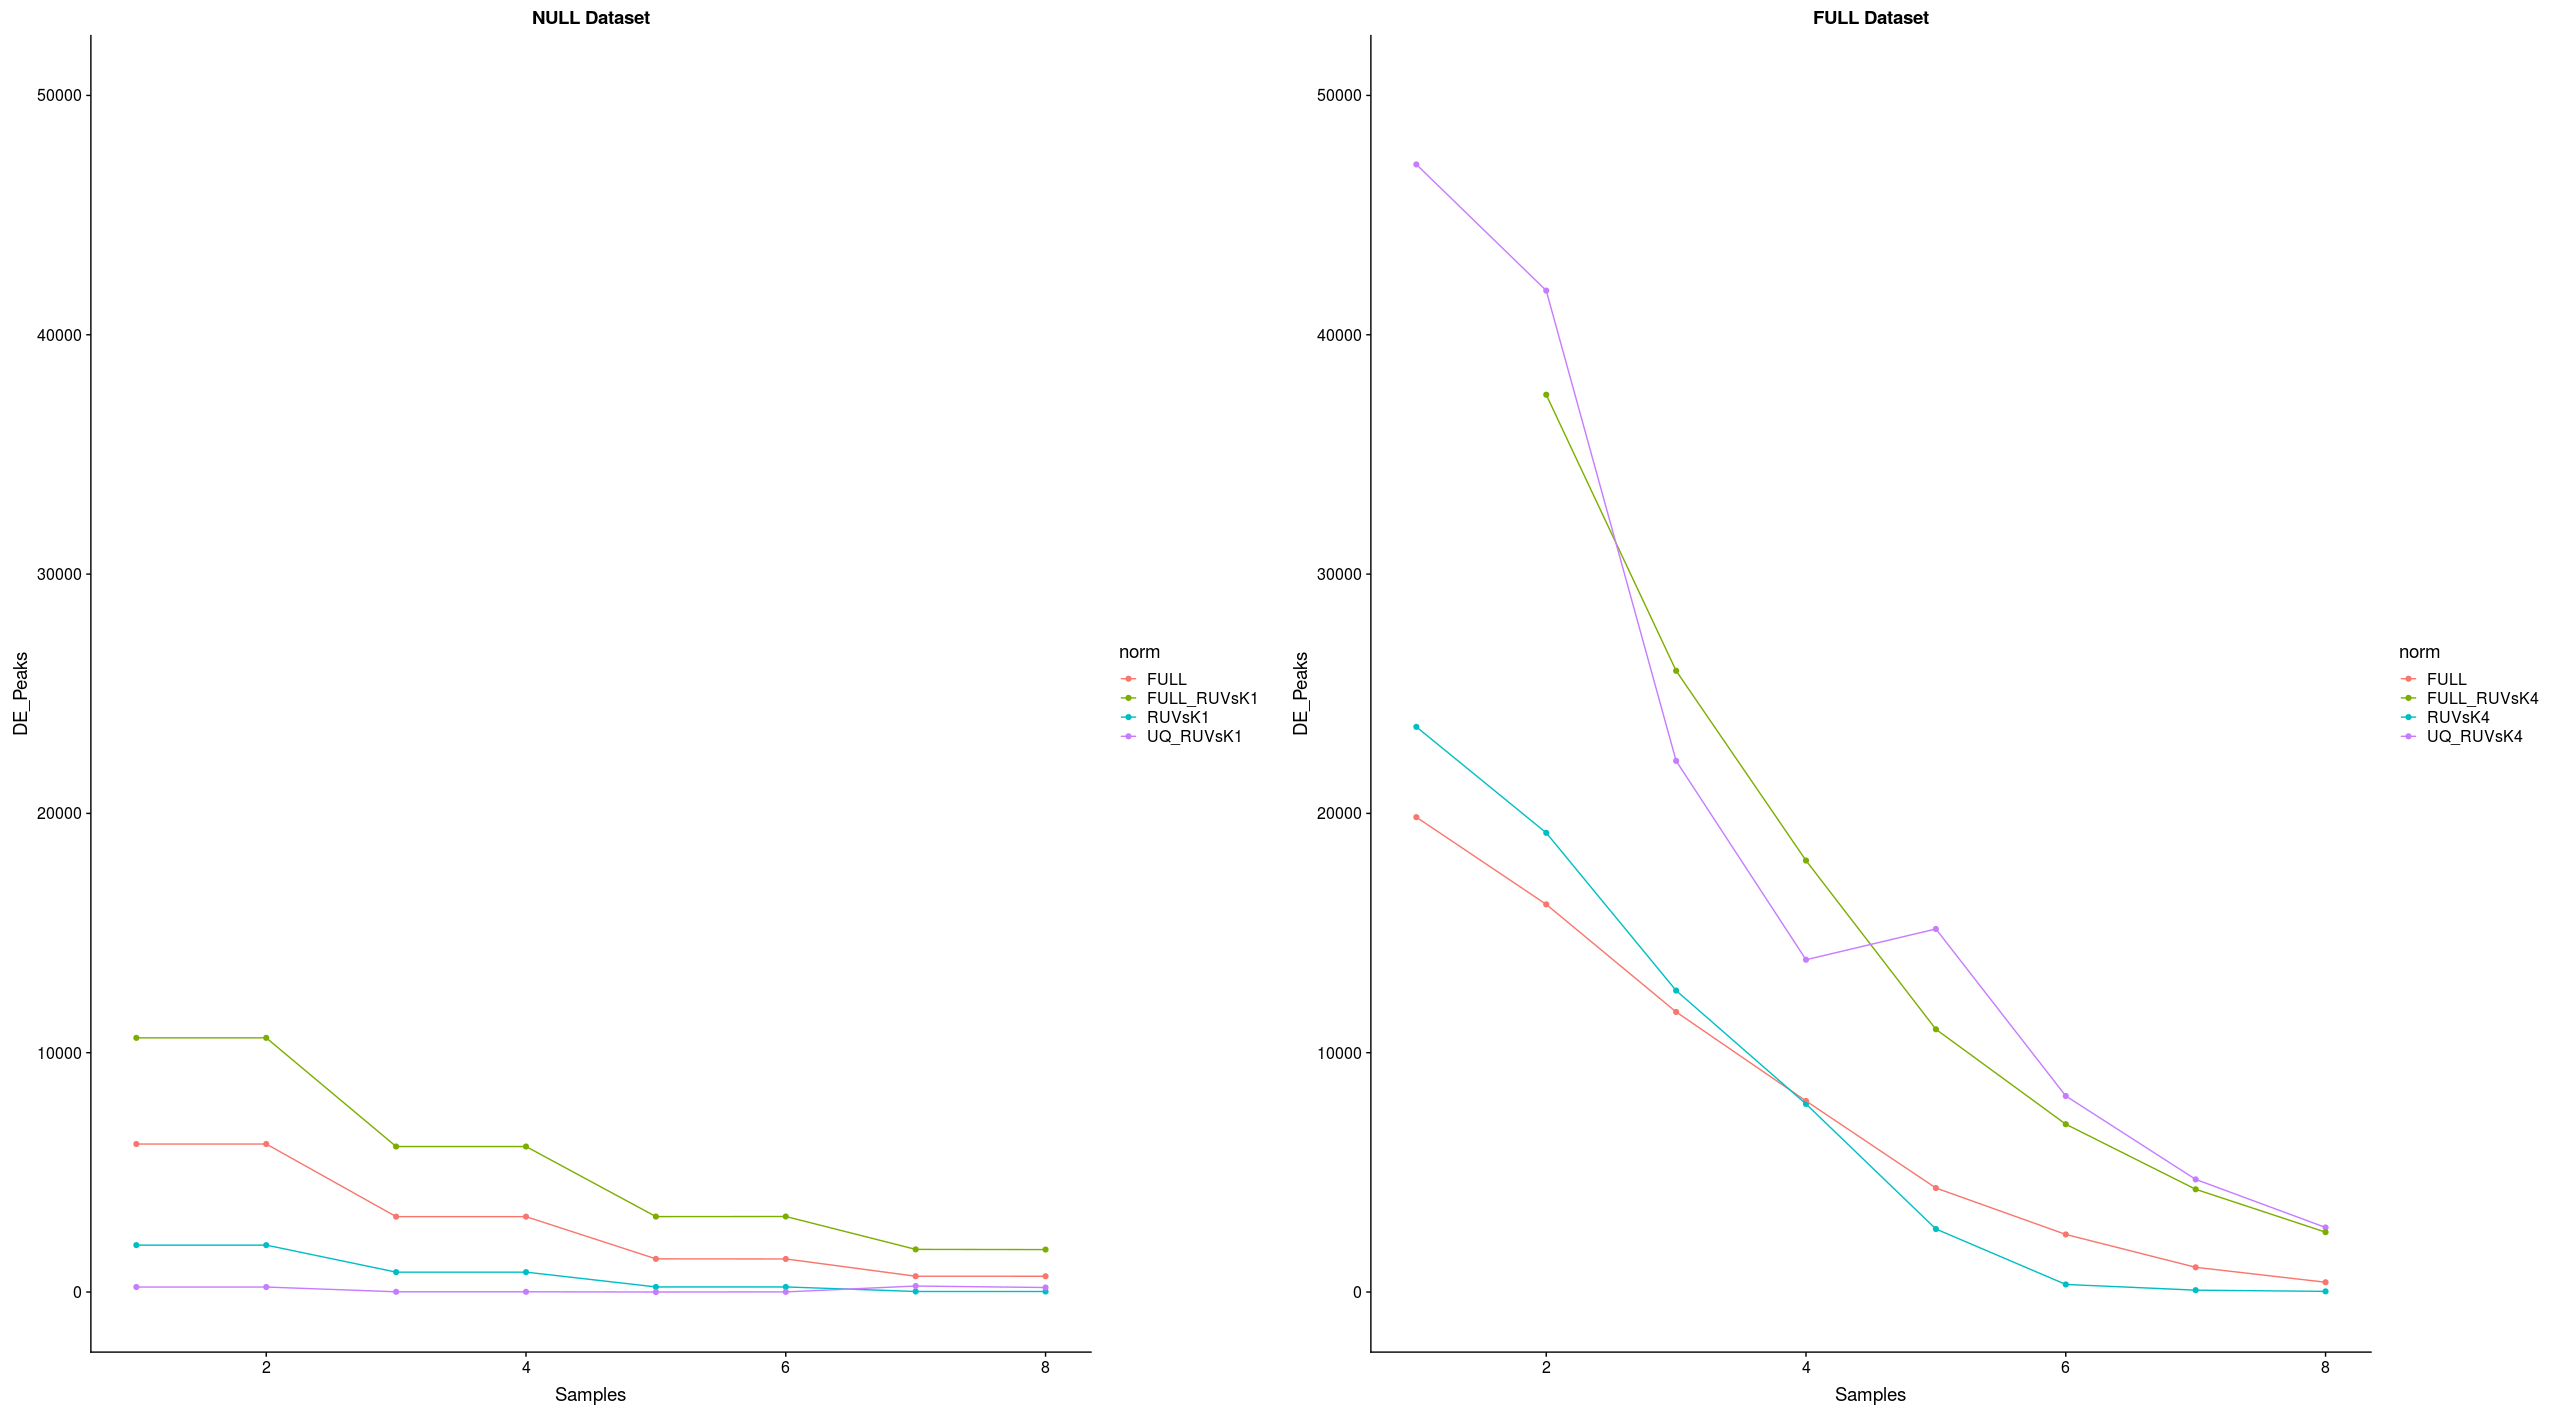
\includegraphics[width=\textwidth, height=\textheight, keepaspectratio]{img/descan2/normalizations_null_full.png}
\caption[Normalizations applied to detected regions]{The figure shows the effects of different normalizations on the epigenomic differentially enriched regions.}
\label{fig:normalizationsnullfull}
\centering
\end{figure}

Even if these normalization methods show good performances with this type of epignomic data, our investigations suggest that more testing is required, and maybe an ad-hoc normalization method for these data has to be developed.

The left panel represent the "null dataset" highlighting that portion of \glspl{der} due to randomness/bias. Indeed, any kid of normalization produces almost the same trend, underlying that \textit{full quantile}, even if combined with \textit{RUV-Seq} still not reduces the bias.
While \textit{upper quartile} preserves oscillations when using 7/8 samples.
The one which seems to well interpret the data, producing a good compromise between bias and signal, is RUV-Seq.
Indeed, it preserves a gradually downhill of the \gls{der} without totally flatten the signal.

A note to be accounted is that in the case of the "null dataset" we had to set the RUV-Seq \lstinline!k! parameter to 1, otherwhise we were no able to obtain any result.
%\begin{figure}[H]
%\centering
%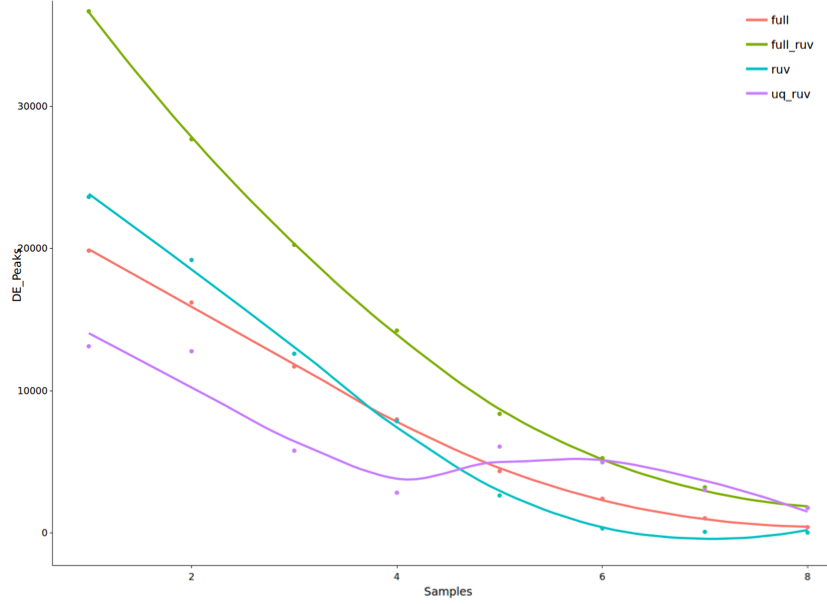
\includegraphics[width=\textwidth, height=\textheight, keepaspectratio]{img/descan2/normalizations.png}
%\caption[Normalizations applied to detected regions]{The figure shows the effects of different normalizations on the epigenomic differentially enriched regions.}
%\label{fig:normalizationsdescan}
%\centering
%\end{figure}
\subsubsection{Differential Enrichment of Peaks}

To estimate the \glspl{der}, any of the RNA-Seq methods can be applied, such as \textit{DESeq2}, \textit{edgeR}, \textit{NOISeq}, etc \cite{Robinson2009, McCarthy2012, Tarazona2012}.

\begin{figure}[H]
\centering
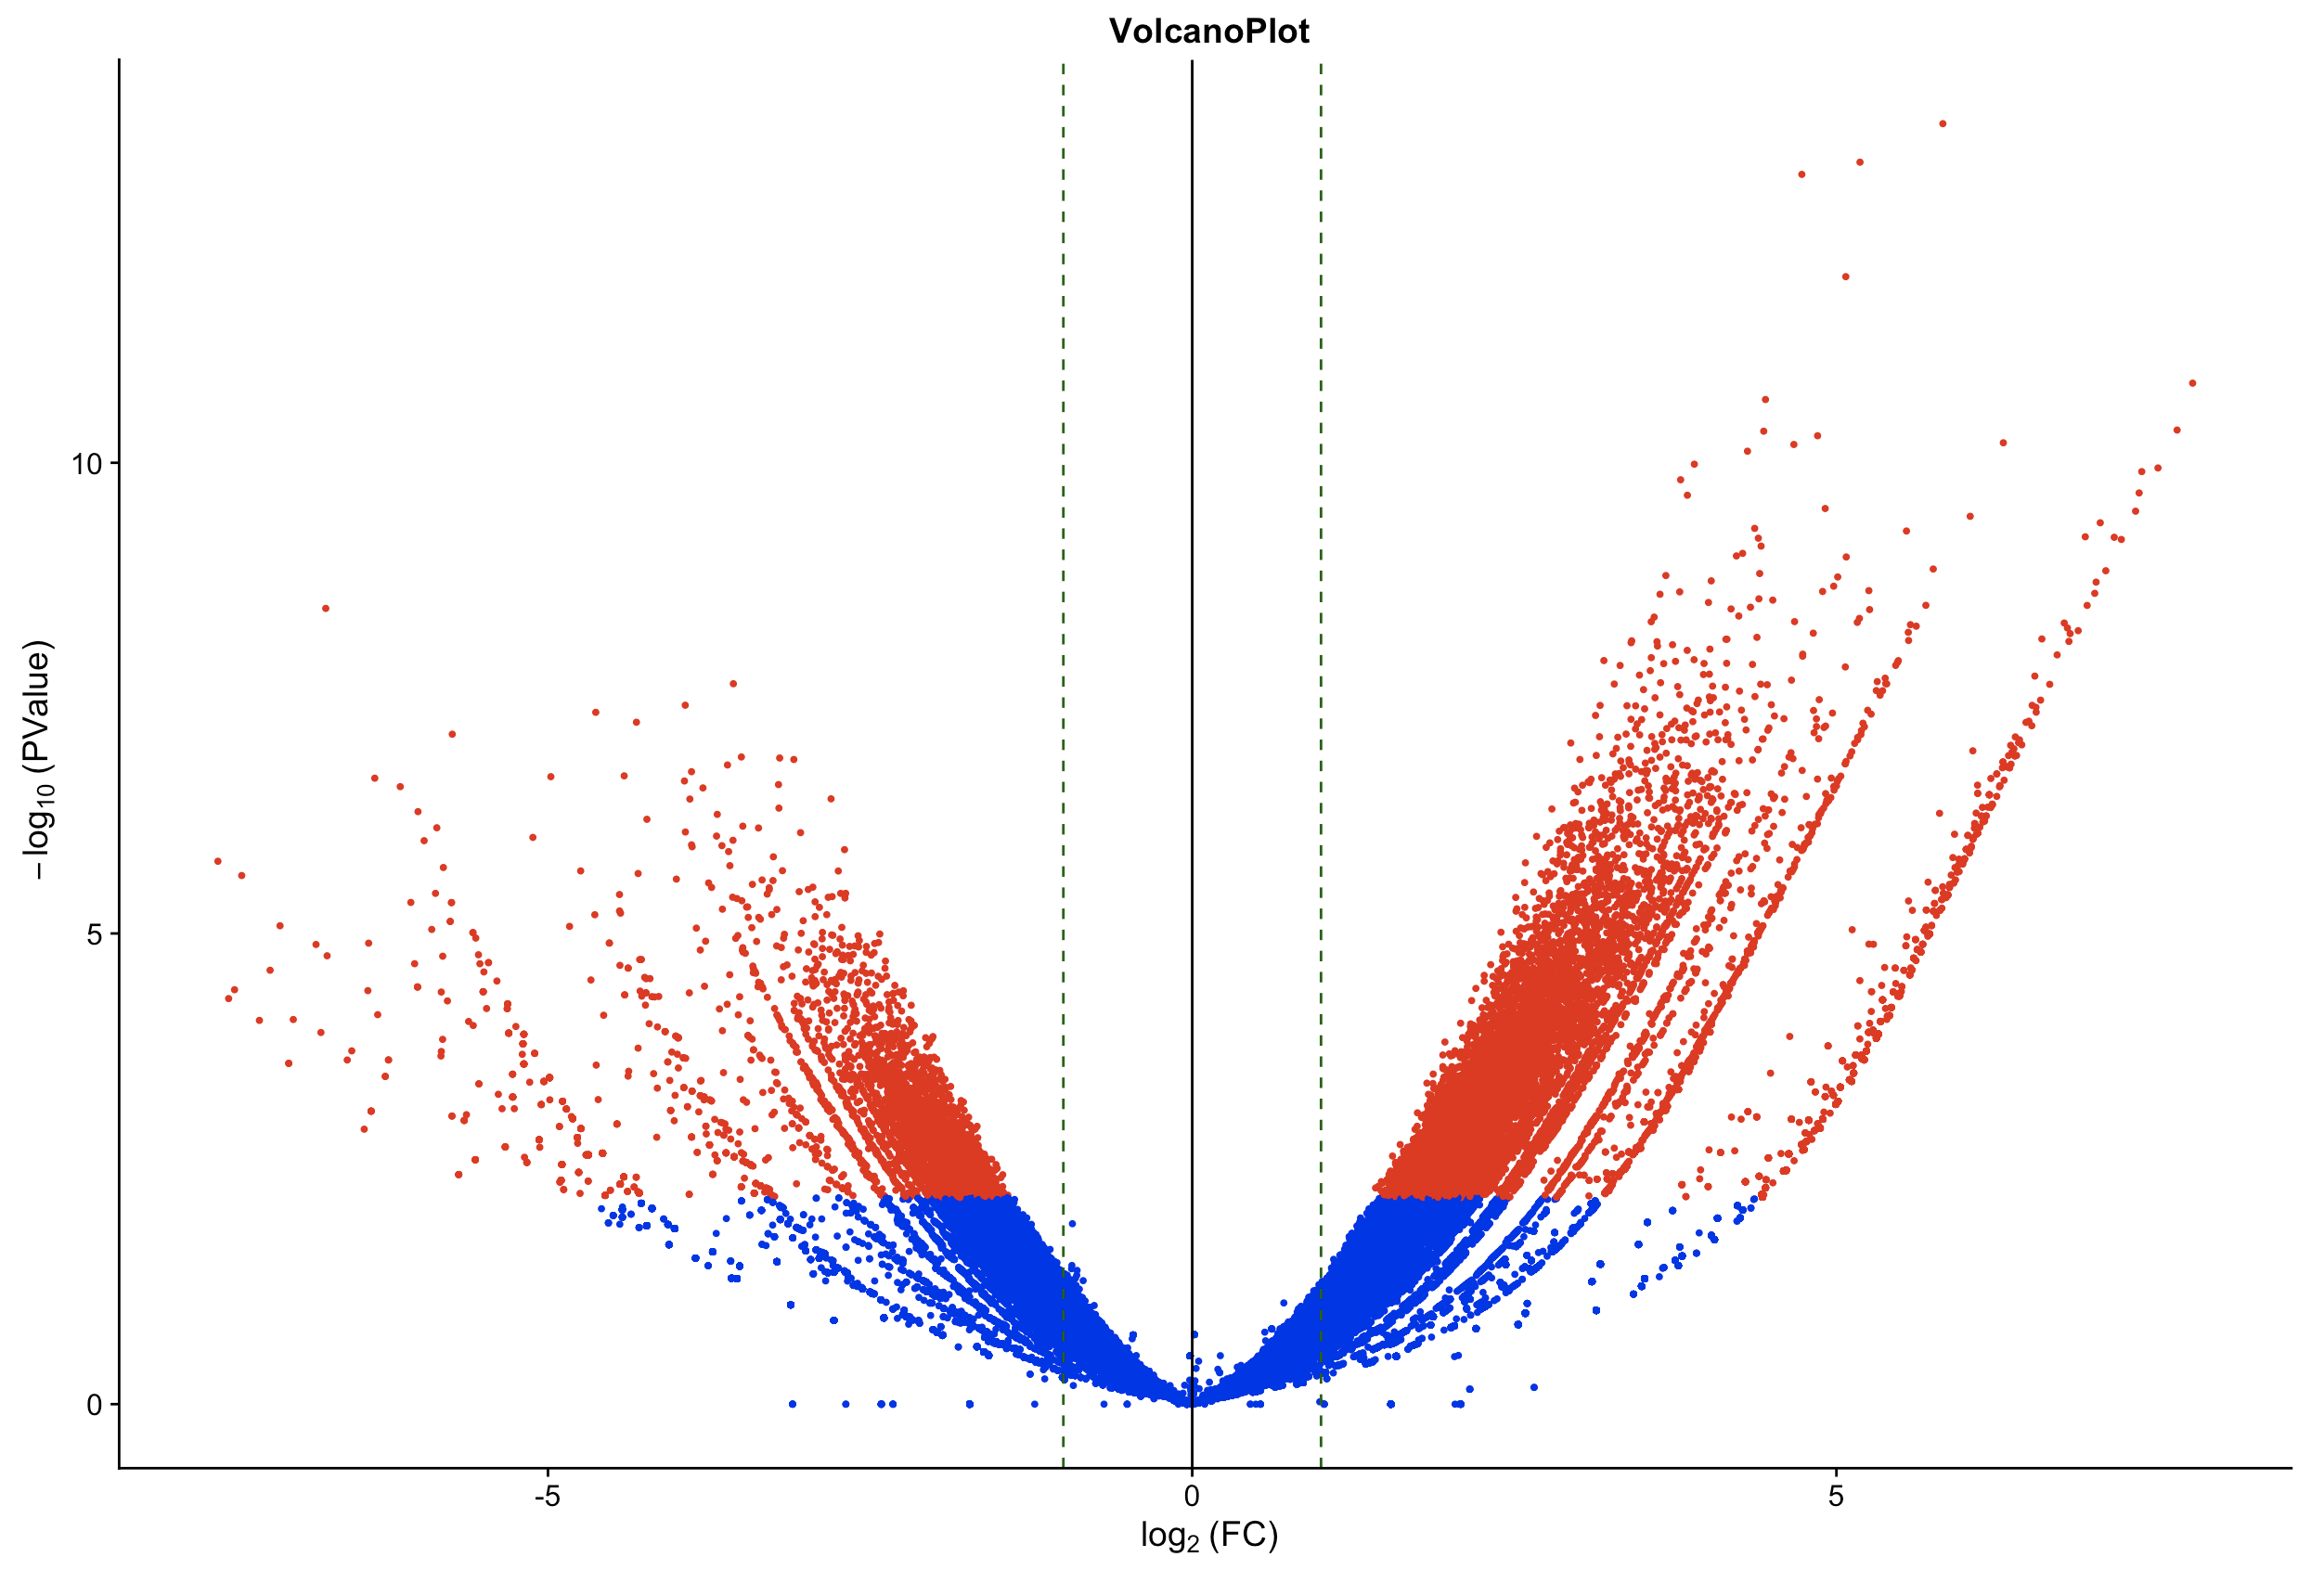
\includegraphics[width=\textwidth, height=\textheight, keepaspectratio]{img/descan2/DE_peaks.png}
\caption[Differential Enrichment Regions Volcano]{A volcano plot of Differential Enriched Regions. Blue dots represent the not significant \glspl{der}, while the red ones represent the significant \glspl{der}.}
\label{fig:depeaksdescan}
\centering
\end{figure}

In this case, we decided to use \textit{edgeR} package, because of its wide range of  available statistical approaches and the possibility to better tune the design of the experiment. 
Indeed, because we used the RUV-Seq normalized counts with \lstinline!k! parameter set to 4, we modeled the experimental design with the \lstinline!model.matrix! function, adding to our model not only the experimental conditions, but also the RUV-Seq estimated weights.
Then we used the resulted design to estimate the dispersion and fit a Quasi-Likelihood test, as defined in edgeR\cite{Robinson2009}.
 
\begin{figure}[H]
\centering
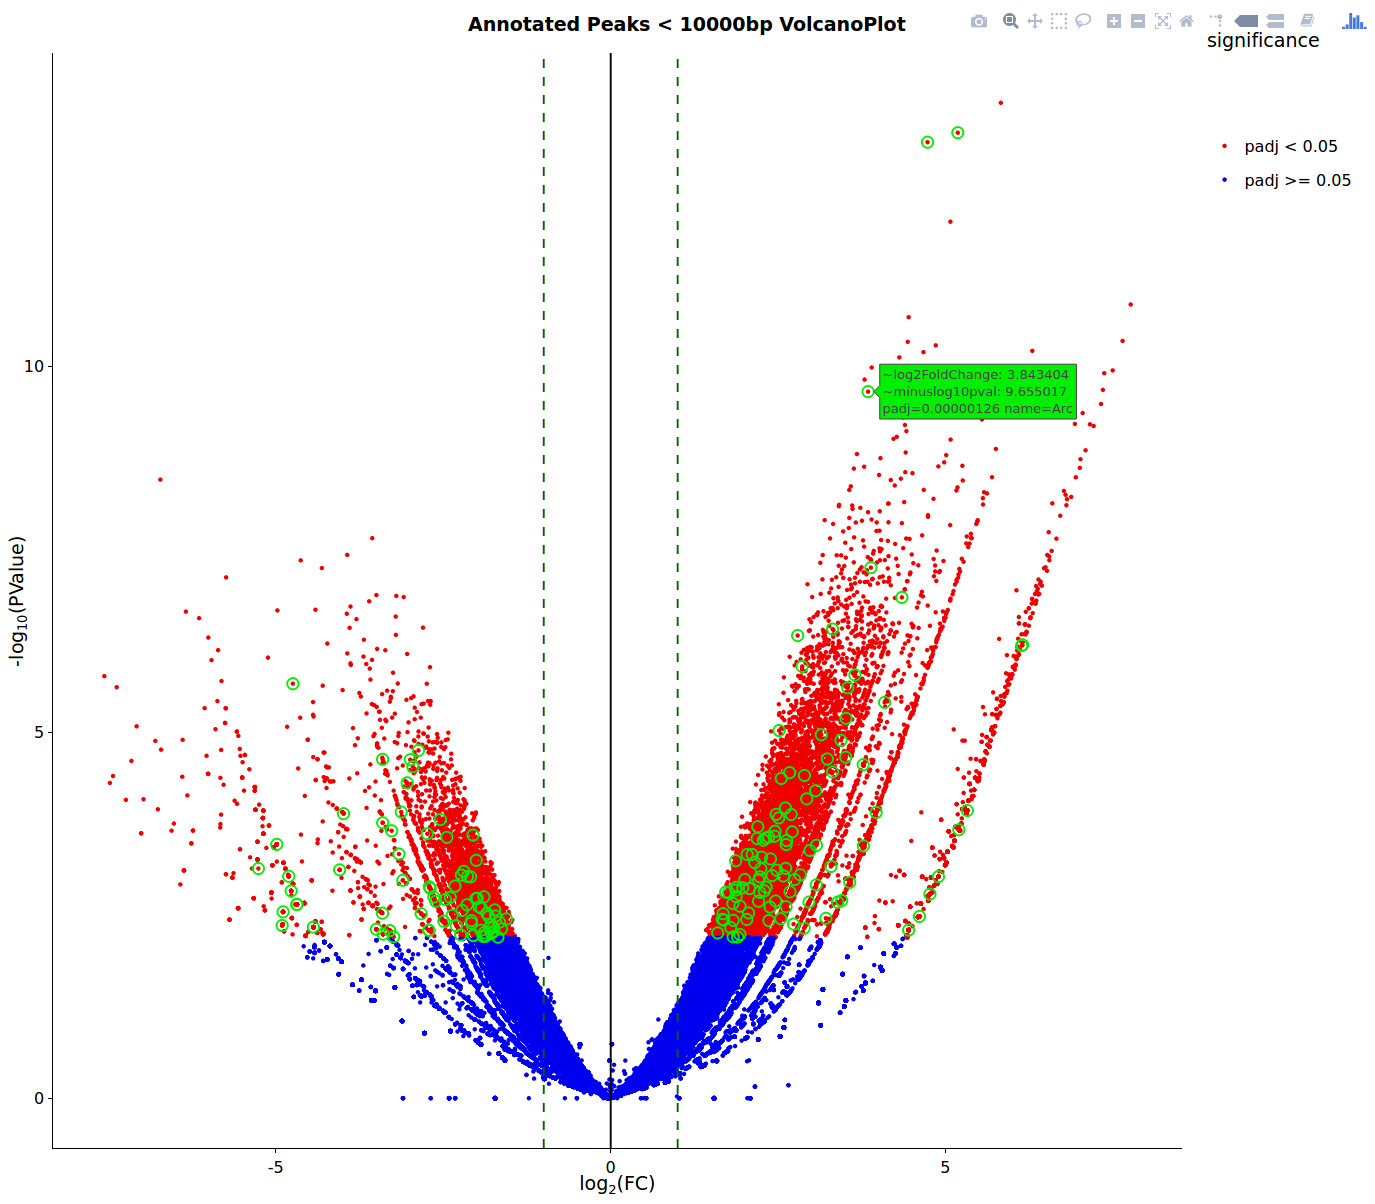
\includegraphics[width=\textwidth, height=\textheight, keepaspectratio]{img/descan2/Annotated_depeaks_degenes.png}
\caption[Annotated Differential Enrichment Regions Volcano]{A volcano plot of \glspl{der}. Blue dots represent the not significant \glspl{der}, while the red ones represent the significant \glspl{der}. Green circles highlights the peaks with a \gls{deg} annotated.}
\label{fig:depeakdegenessdescan}
\centering
\end{figure}

The figure \ref{fig:depeaksdescan} shows a volcano plot of \glspl{der} between E0 and E1 conditions.
Red dots highlights the regions with a \gls{fdr}\cite{Benjamini1995} lower than 0.05, while blue dots highlight not significant regions.

\subsubsection{Peaks Integration}

Next task is to integrate the obtained results with other omic data types, as RNA-Seq. 
Because of the low number of the samples, the easiest way to integrate the data is to annotate the \glspl{der} with \glspl{deg} resulting from the analysis of RNA-Seq.

For the differential expression of the RNA-Seq data we firstly quantified the signal with \lstinline!featureCounts! methods available in the \textit{Rsubread} \cite{Liao2013} R/Bioconductor package.
Then we filtered lowly expressed genes with the \textit{proportion} test  as implemented in \textit{NOISeq} package, and applied the \lstinline!noiseq! method for differential expression.

We used the resulting significant \glspl{deg} (with posterior probability higher than 0.95) to annotate the peaks with \lstinline!annotatePeakInBatch! method of \textit{ChIPpeakAnno}.
Figure 	\ref{fig:depeakdegenessdescan} illustrates with green circles the peaks with an annotated gene with distance lower than 10000bp from the gene \gls{tss}, producing a total of 430 annotated peaks.
Realizing the plot with \textit{ggplot2} combined with \textit{plotly} library it is possible to enhance the names of the genes with a tooltip.

Then we used the annotated genes to do functional annotation on \gls{go} \cite{GeneOntologyConsortium2004, GeneOntologyConsortium2015} and Reactome pathways, which showed several interesting results for the neuronal regulation.

\textbf{Insert tables for the functional results, to discuss with Davide/Lucia}







